\section{Lois continues}
    \subsection{Loi Uniforme sur $[0,1]$, notée $\mathbb{U}([0,1])$}
        On dit que $X$ suit une loi uniforme sur $[0,1]$ ssi sa fonction densité est : 
        \begin{equation}
            f_X(x) = \left\{
                \begin{array}{ll}
                    1 & \text{si } x \in [0,1] \\
                    0 & \text{sinon}
                \end{array}
            \right.
        \label{eq:loi_uniforme_01}
        \end{equation}

    La fonction de répartition d’une loi uniforme sur $[0,1]$ est :
    \begin{equation}
        \forall x\in\mathbb R,\, F(x)=\int_{-\infty}^x f(t)\,dt = \left\{
            \begin{array}{ll}
                0 & \text{si } x < 0 \\
                x & \text{si } x \in [0,1] \\
                1 & \text{si } x > 1
            \end{array}
        \right.
    \end{equation}

    L’espérance de la loi uniforme $U_{[0,1]}$ est $\mathbb{E}[X]=\frac{1}{2}$. Le moment d’ordre 2 est $\mathbb{E}[X^2]=\frac{1}{3}$ et la variance est $\mathbb{V}[X]=\frac{1}{12}$ (voir \cite{loi_uniforme}). 
    
    \subsubsection{Exemple - Simulation de la loi uniforme sur $[0,1]$}
        \textbf{Voir code GitHub \cite{git} : Section 3.1 Loi uniforme sur $[0,1]$}

        \begin{figure}[H]
            \centering
            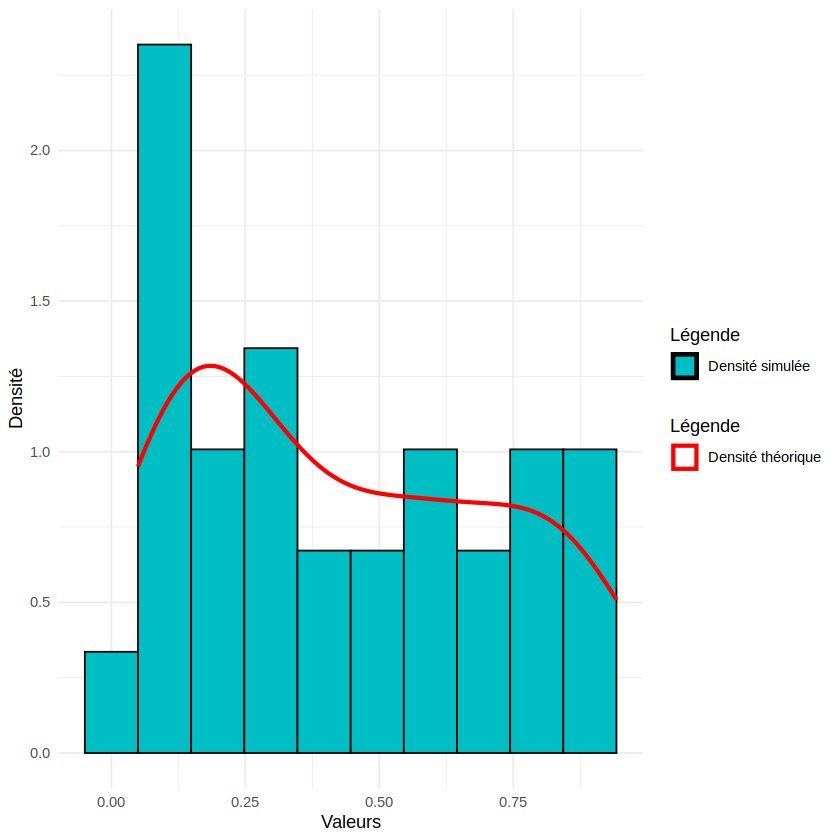
\includegraphics[width=0.23\textwidth]{4_attachments/figures/output8.png}
            \caption{Histogramme de simualtion par loi uniforme sur $[0,1]$ avec sa courbe de densité}
            \label{fig:histogramme_uniforme_01}
        \end{figure}

    \subsubsection{Analyse des résultats}
        La figure \ref{fig:histogramme_uniforme_01} montre un histogramme de simulation $S$ de la loi uniforme sur $[0,1]$ avec sa courbe de densité. 
        L'histogramme montre que les valeurs générées tendent à être réparties uniformément sur l'intervalle $[0,1]$ et que sa courbe de densité tend à être constante et égale à 1 (voir \ref{eq:loi_uniforme_01}).

        La moyenne des valeurs par la probabilité d'apparition de cette simulation est : $\mathbb{E}[S] = 0.426$ et la variance est : $\mathbb{V}[S] = 0.083$. D'après les valeurs théoriques, on a $\mathbb{E}[X] = \frac{1}{2} \approx \mathbb{E}[S]$ et $\mathbb{V}[X] = \frac{1}{12} \approx \mathbb{V}[S]$. On peut donc conclure que les valeurs simulées sont proches des valeurs théoriques.

    \subsection{Loi Uniforme sur $[a,b]$, notée $\mathbb{U}([a,b])$ avec $a < b$}

        On dit que $X$ suit une loi uniforme sur $[a,b]$ ssi sa fonction densité est : 
        \begin{equation}
            f_X(x) = \left\{
                \begin{array}{ll}
                    \frac{1}{b-a} & \text{si } x \in [a,b] \\
                    0 & \text{sinon}
                \end{array}
            \right.
        \label{eq:loi_uniforme_ab}
        \end{equation}

        La fonction de répartition d’une loi uniforme sur $[a,b]$ est :
        \begin{equation}
            \forall x\in\mathbb R,\, F(x)=\int_{-\infty}^x f(t)\,dt = \left\{
                \begin{array}{ll}
                    0 & \text{si } x < a \\
                    \frac{x-a}{b-a} & \text{si } x \in [a,b] \\
                    1 & \text{si } x > b
                \end{array}
            \right.
        \end{equation}

        L’espérance de la loi uniforme $U_{[a,b]}$ est $\mathbb{E}[X]=\frac{a+b}{2}$. Le moment d’ordre 2 est $\mathbb{E}[X^2]=\frac{a^2+ab+b^2}{3}$ et la variance est $\mathbb{V}[X]=\frac{(b-a)^2}{12}$ (voir \cite{loi_uniforme}).

        \subsubsection{Exemple - Simulation de la loi uniforme sur $[a,b]$}
        \textbf{Voir code GitHub \cite{git} : Section 3.2 Loi uniforme sur $[a,b]$}

        \begin{figure}[H]
            \centering
            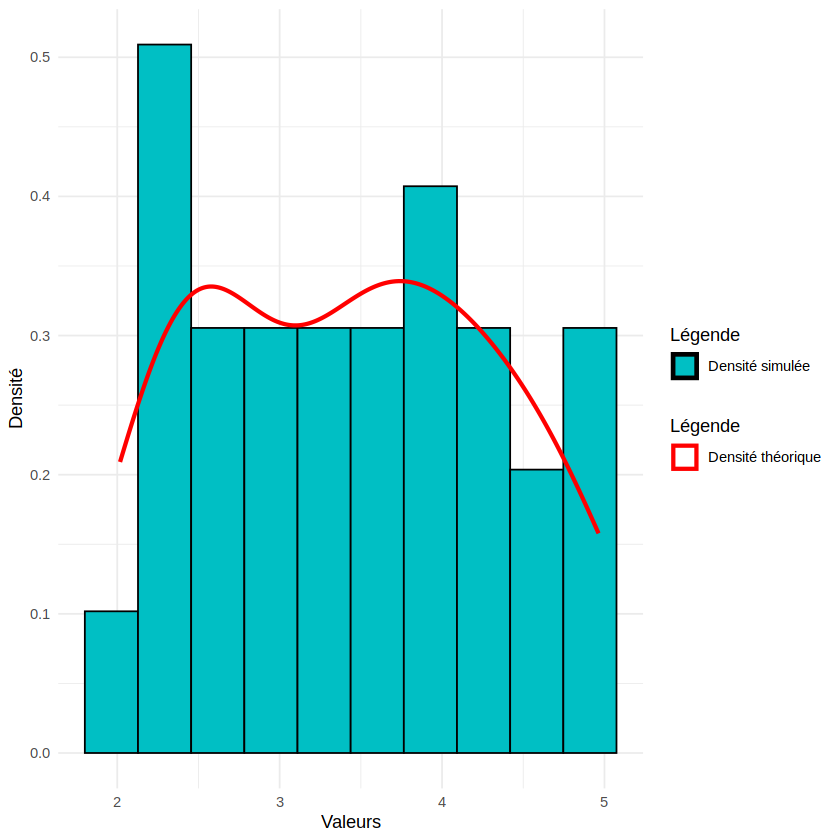
\includegraphics[width=0.23\textwidth]{4_attachments/figures/output9.png}
            \caption{Histogramme de simualtion par loi uniforme sur $[2,5]$ avec sa courbe de densité}
            \label{fig:histogramme_uniforme_ab}
        \end{figure}

        \subsubsection{Analyse des résultats}
        La figure \ref{fig:histogramme_uniforme_ab} montre un histogramme de simulation $S$ de la loi uniforme sur $[2,5]$ avec sa courbe de densité. 
        L'histogramme montre que les valeurs générées tendent à être réparties uniformément sur l'intervalle $[2,5]$ et que sa courbe de densité tend à être constante et égale à $\frac{1}{3}$ car $\frac{1}{b-a} = \frac{1}{5-2}$ (voir équation \ref{eq:loi_uniforme_ab}).       
        
        La moyenne des valeurs par la probabilité d'apparition de cette simulation est : $\mathbb{E}[S] = 3.421$ et la variance est : $\mathbb{V}[S] = 0.805$. D'après les valeurs théoriques, on a 
        
        \[
        \mathbb{E}[X] = \frac{a+b}{2} = \frac{5+2}{2} = 3.5 \approx \mathbb{E}[S]
        \]
        \[
        \mathbb{V}[X] = \frac{(b-a)^2}{12} = \frac{(5-2)^2}{12} = 0.75 \approx \mathbb{V}[S]
        \]
        On peut donc conclure que les valeurs simulées sont proches des valeurs théoriques.



    \subsection{Loi Normale centrée réduite, notée $\mathcal{N}(0,1)$}
        Si $X\leadsto\mathcal N(0,1)$ alors la fonction densité de $X$ est :
        \begin{equation}
            \forall x\in\mathbb R,\, f(x)= \dfrac{1}{\sqrt{2\pi}}e^{-\frac{x^2}{2}}
        \end{equation}

        L'espérance de la loi normale centrée réduite est $\mathbb{E}[X]=0$ et la variance est $\mathbb{V}[X]=1$ (voir \cite{loi_normale}).

        \subsubsection{Exemple - Simulation de la loi normale centrée réduite $\mathcal N(0,1)$}
        \textbf{Voir code GitHub \cite{git} : Section 3.3 Loi Normale centrée réduite notée $\mathcal N(0,1)$}
        \begin{figure}[H]
            \centering
            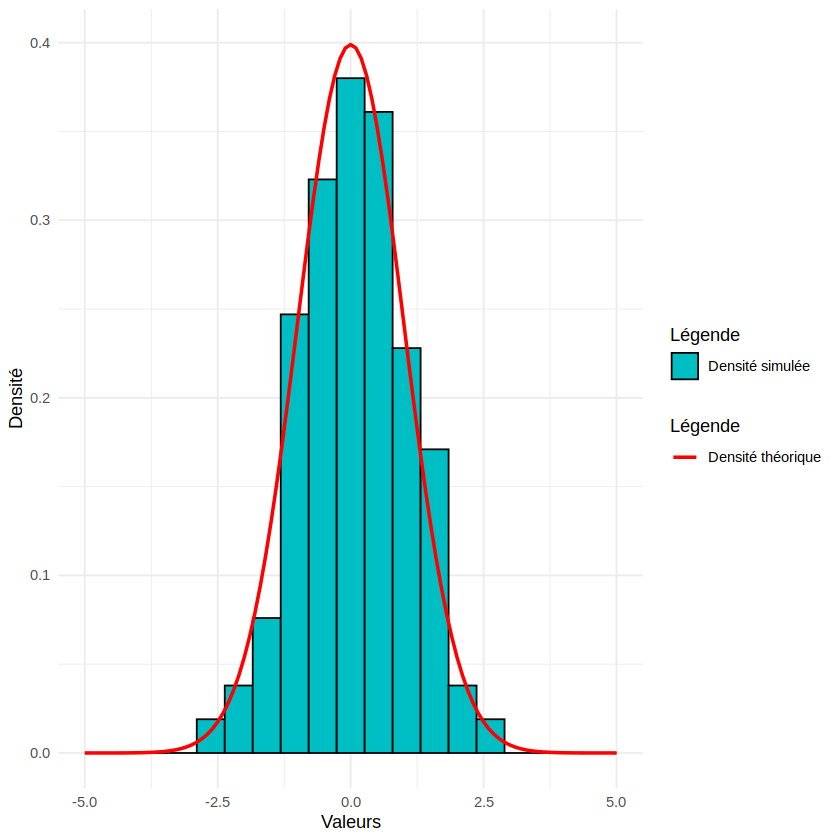
\includegraphics[width=0.35\textwidth]{4_attachments/figures/output10.png}
            \caption{Histogramme de simualtion par loi normale centrée réduite $\mathcal N(0,1)$ avec la courbe de densité théorique}
            \label{fig:histogramme_normale_01}
        \end{figure}

        \subsubsection{Analyse des résultats}
            La figure \ref{fig:histogramme_normale_01} illustre la distribution d'une loi normale centrée réduite, laquelle est symétrique par rapport à $x=0$, son point de densité maximale, et décroît de part et d'autre. 
            En analysant la moyenne et la variance de la simulation $S$ représenté sous forme d'histogramme, nous obtenons :
            \[
                \mathbb{E}[S] = 0.07 \approx \mathbb{E}[X] = 0
                \]
                \[
                \mathbb{V}[S] = 1.02 \approx \mathbb{V}[X] = 1
            \]
            La symétrie autour de $x=0$ s'explique par le paramètre $\mu=0$ (moyenne) de la distribution. L'variance, quant à lui, détermine la dispersion des valeurs autour de la moyenne, influençant ainsi la forme de la courbe de densité.

        \subsubsection{Démonstration}
            La proposition de départ est : 
            \begin{equation}
                \mathbf{\int_{-\infty}^{+\infty}e^{-\dfrac{x^2}{2}}\,dx=\sqrt{2\pi}}
            \end{equation}

            \begin{enumerate}
                \item Nous savons que $\sqrt{2\pi} = 2.506628$. Il est possible de simuler cette equation sur $R$ (\textbf{voir code annexe \ref{lst:comparaison}}). En utilisant avec la fonction $interval$ nous obtenons : $2.506628$ avec une erreur absolue $< 0.00023$.Ce qui confirme la proposition de départ.
                \item Nous pouvons également comparer graphiquement les 2 equations, voir figure \ref{fig:egalite} et nous remarquons que les 2 courbes se superposent parfaitement.
            \end{enumerate}
            \begin{figure}[H]
                \centering
                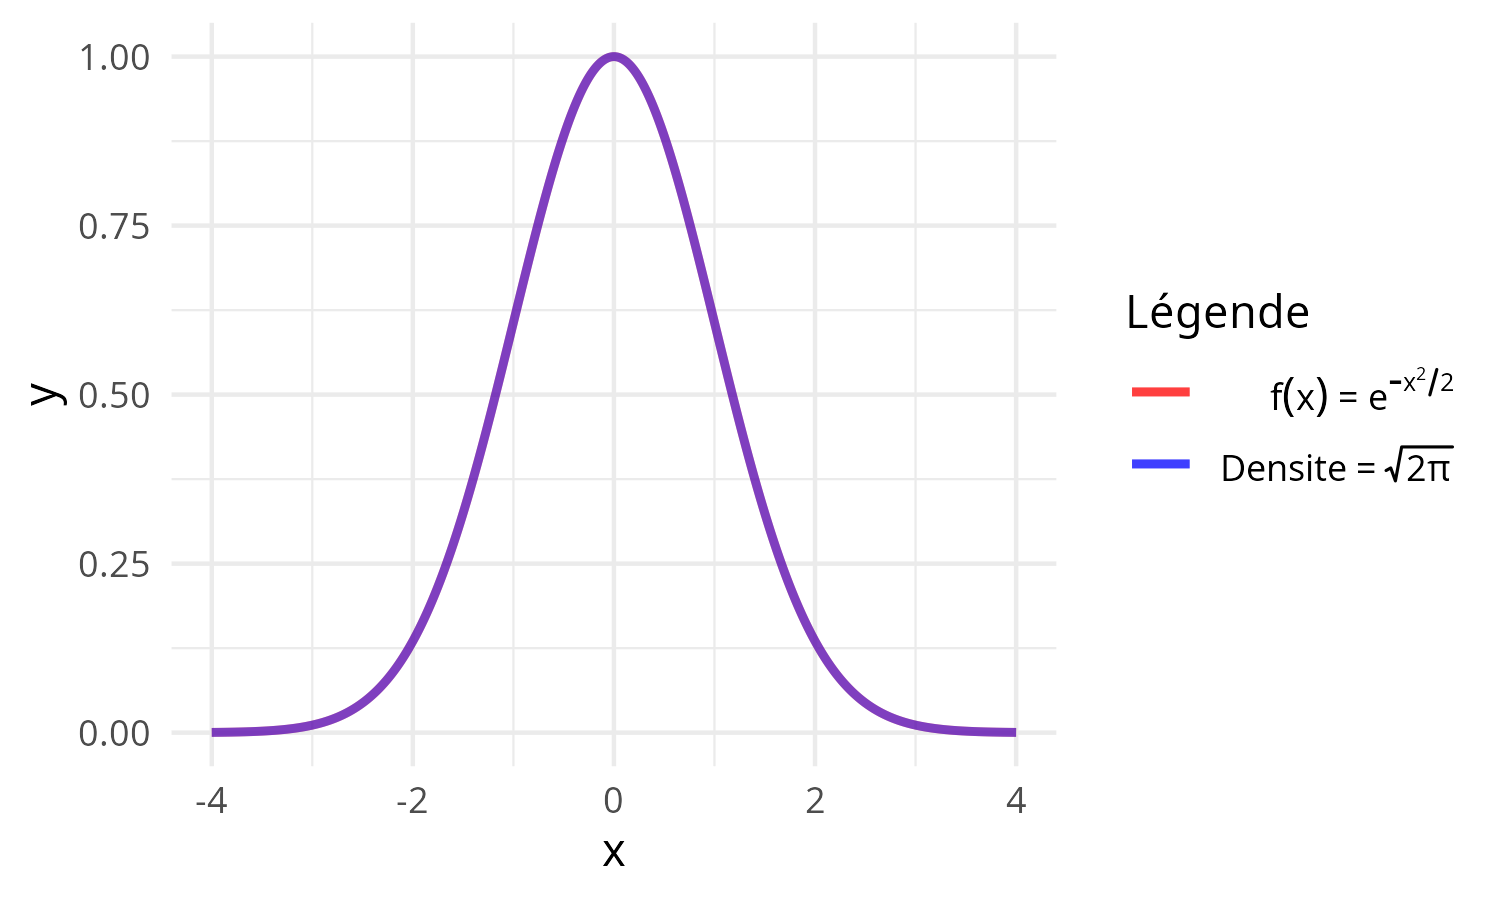
\includegraphics[width=0.28\textwidth]{4_attachments/figures/output11.png}
                \caption{Comparaison graphique des 2 équations (Voir Code Github : section 3.4 \cite{git})}
                \label{fig:egalite}
            \end{figure}


    \subsection{Loi Normale, notée $\mathcal{N}(\mu,\sigma^2)$}
        Si $X\leadsto\mathcal N(\mu,\sigma^2)$ alors la fonction densité de $X$ est :

        \begin{equation}
            \forall x\in\mathbb R,\, f(x)= \dfrac{1}{\sigma\sqrt{2\pi}}e^{-\frac{(x-\mu)^2}{2\sigma^2}}
        \end{equation}

        \subsubsection{Exemple - Simulation de la loi normale centrée réduite $\mathcal N(1,4)$}
        Voir code TP : Section Loi Normale $\mathcal{N}(\mu,\sigma^2)$ \cite{TP}
        \begin{figure}[H]
            \centering
            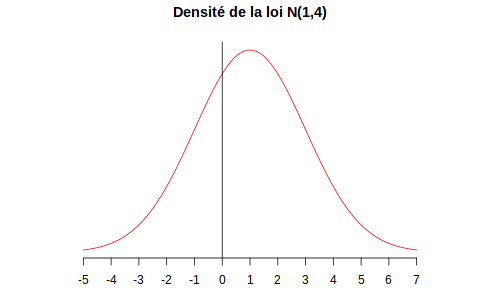
\includegraphics[width=0.3\textwidth]{4_attachments/figures/output12.png}
            \caption{Histogramme de simualtion par loi normale centrée réduite $\mathcal N(1,4)$}
            \label{fig:histogramme_uniforme_ab}
        \end{figure}

        \subsubsection{Analyse des résultats}
            Le graphique de la figure \ref{fig:histogramme_uniforme_ab} suit une loi normale centrée réduite, $\mathcal N(1,4)$ laquelle est symétrique par rapport à $x=1=\mu$, son point de densité maximale. 
            Et $\sigma = 4$ détermine la dispersion des valeurs autour de la moyenne, influençant ainsi la forme de la courbe de densité. Elle parrait donc plus applatie.
        \subsection{Théorème}
            \begin{equation}
                \text{Si } \mathbf{X\leadsto\mathcal N(\mu,\sigma^2)} \text{ alors } \mathbf{\dfrac{X-\mu}\sigma\leadsto\mathcal N(0,1)}
            \end{equation}

            Pour vérifier le théorème, il faut tracer un graphique (voir figure \ref{fig:theoreme}) de la loi normale centrée réduite $\mathcal N(0,1)$ et de la loi normale $\mathcal N(1,4)$ centrée en $\mu=1$ et d'variance $\sigma^2=4$.
            Dans la figure ci dessous, les 2 courbes de denstité tendent à se supperposer pour un échantillon de taile $n=2000$. (\textbf{voir code annexe \ref{lst:theoreme}})

            \begin{figure}[H]
                \centering
                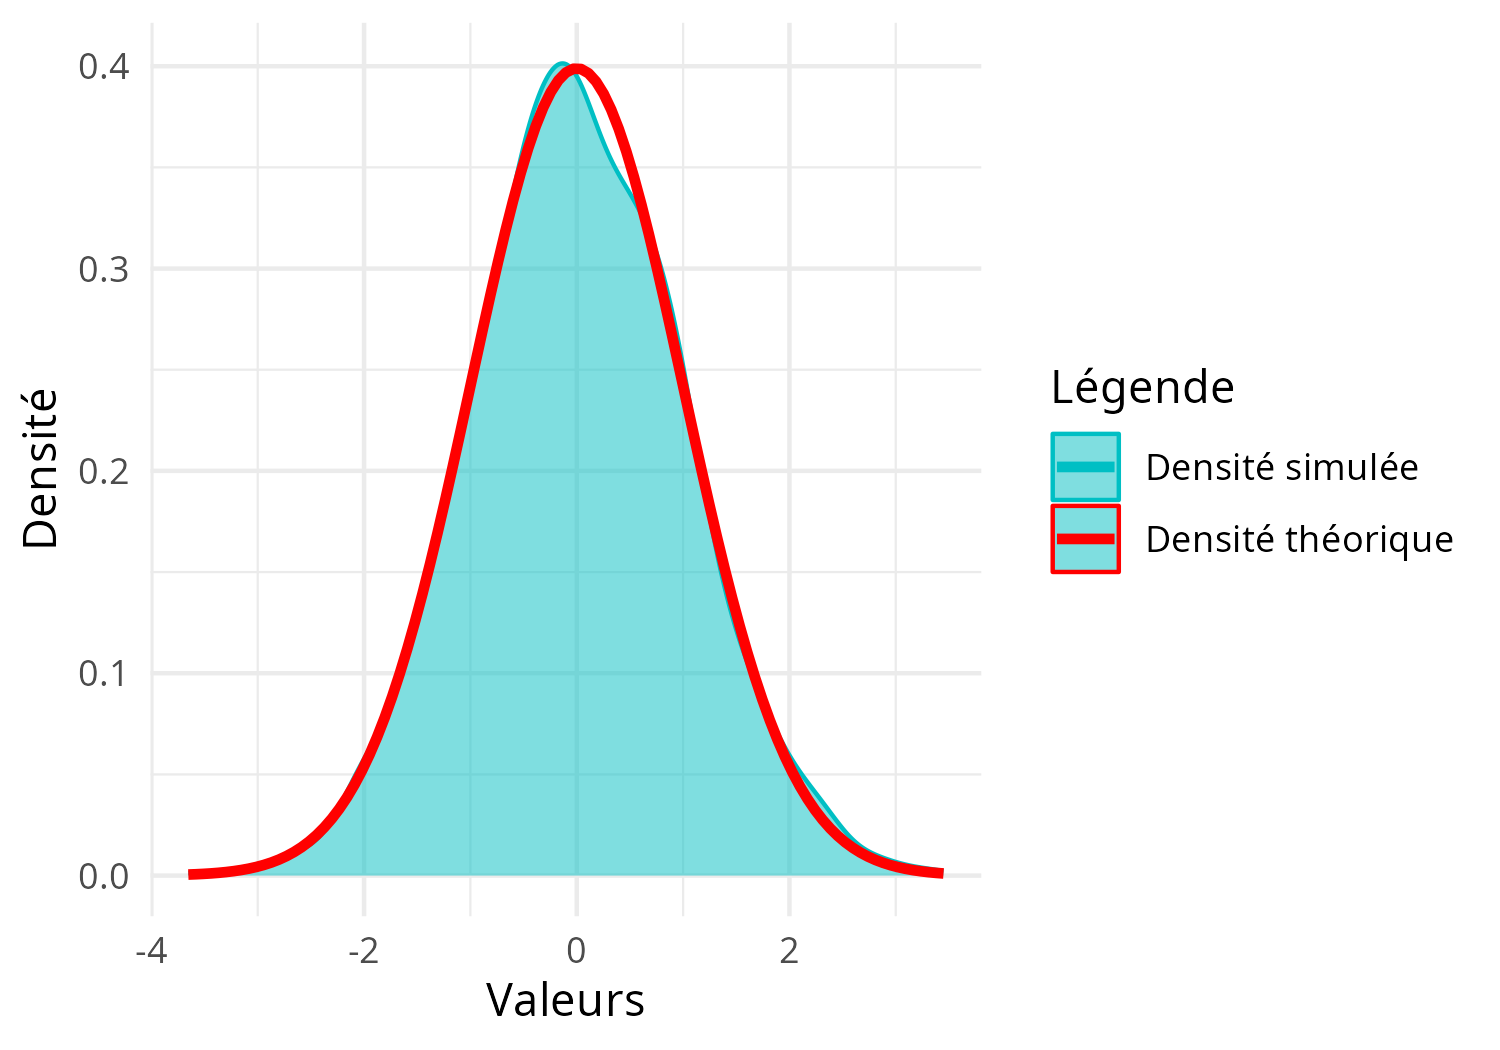
\includegraphics[width=0.3\textwidth]{4_attachments/figures/reduced_plot.png}
                \caption{Comparaison des courbes de densité de la loi normale centrée réduite $\mathcal N(0,1)$ et de la loi normale $\mathcal N(1,4)$ centrée en $\mu=1$ et d'variance $\sigma^2=4$}
                \label{fig:theoreme}
            \end{figure}


    \subsection{Exercices sur la loi normale}
        Pour simuler $n$ valeurs aléatoirement suivant la loi normale de moyenne $m$ et d’variance $s$ on utilise sous R la commande \textbf{rnorm}.
        Nous avons effectuez 5 simulation de la oi normal d'une taille $n=20$ et de paramètres : $\mathcal N(0,1)$, $\mathcal N(1,1)$, $\mathcal N(2,1)$, $\mathcal N(0,2)$, $\mathcal N(0,4)$.
        Voici ci-dessous le tableau résultant de ces simulations:

        \begin{table}[H]
            \centering
            \begin{tabular}{|c|c|c|c|c|c|}
                \hline
                $n=20$&$\mathcal N(0,1)$&$\mathcal N(1,1)$&$\mathcal N(2,1)$&$\mathcal N(0,2)$&$\mathcal N(0,4)$ \\ 
                \hline
                nb de valeurs $< -2$ & 1 & 0 & 0 & 4 & 5 \\
                nb de valeurs $< 0$ & 12 & 3 & 0 & 11 & 10 \\
                nb de valeurs $= 0$ & 0 & 0 & 0 & 0 & 0 \\
                nb de valeurs $> 2$ & 1 & 1 & 11 & 3 & 5 \\
                \hline
            \end{tabular}
            \caption{Tableau de simulation des 5 lois normales de taille $n=20$}
            \label{tab:tab1}
        \end{table}

        \subsubsection{Question 1 : Voir Code TP, section : Exercices sur la loi normale, Question 1 \cite{TP}}
            \begin{center}
                \textit{Avec les mêmes valeurs des moyennes et des variances, on simule maintenant des échantillons de taille n=2000 individus:}
            \end{center}

              \begin{table}[H]
                \centering
                \begin{tabular}{|c|c|c|c|c|c|}
                    \hline
                    $n=20$&$\mathcal N(0,1)$&$\mathcal N(1,1)$&$\mathcal N(2,1)$&$\mathcal N(0,2)$&$\mathcal N(0,4)$ \\ 
                    \hline
                    nb de valeurs $< -2$ & 48 & 4 & 0 & 326 & 595 \\
                    nb de valeurs $< 0$ & 1006 & 308 & 48 & 997 & 978 \\
                    nb de valeurs $= 0$ & 0 & 0 & 0 & 0 & 0 \\
                    nb de valeurs $> 2$ & 55 & 336 & 985 & 319 & 624 \\
                    \hline
                \end{tabular}
                \caption{Tableau de simulation des 5 lois normales de taille $n=2000$ (\textbf{voir code annexe \ref{lst:q1}})}
                \label{tab:tab2}
              \end{table}

        \subsubsection{Question 2: Voir Code TP, section : Exercices sur la loi normale, Question 2 \cite{TP}}
              \begin{center}
                \textit{On considère uniquement le premier échantillon $nd1$. Que trace la fonction plot ?}
              \end{center}
              \begin{table}[H]
                \centering
                \begin{minipage}{0.28\textwidth}
                    \centering
                    \begin{figure}[H]
                        \centering
                        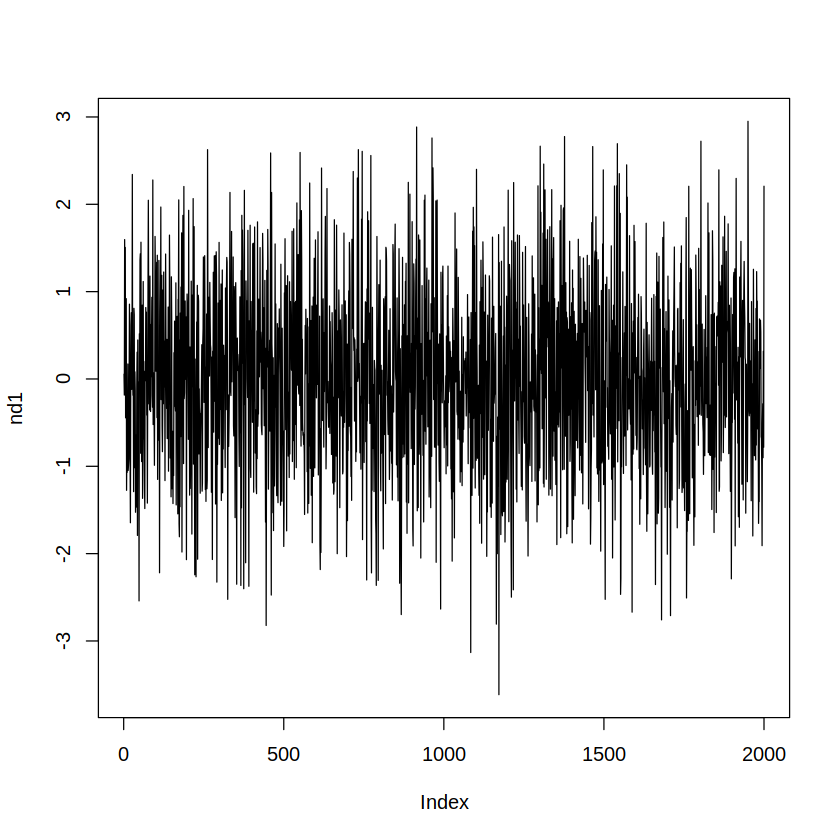
\includegraphics[width=0.7\textwidth]{4_attachments/figures/output21.png}
                        \caption{Graphique en courbe de la loi normale $\mathcal N(0,1)$}
                        \label{fig:fig1}
                    \end{figure}
                
                 \end{minipage}
                \hfill
                \begin{minipage}{0.28\textwidth}
                    \centering
                    \begin{figure}[H]
                        \centering
                        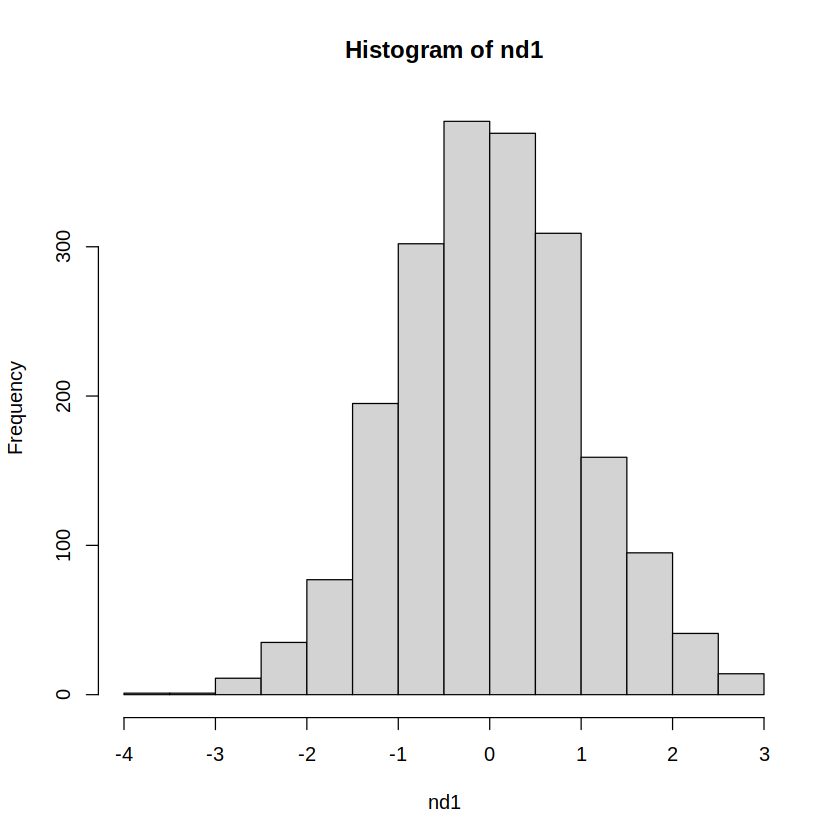
\includegraphics[width=0.7\textwidth]{4_attachments/figures/output22.png}
                        \caption{Histogramme de la loi normale $\mathcal N(0,1)$}
                        \label{fig:fig2}
                    \end{figure}
                    
                \end{minipage}
                \hfill
                \begin{minipage}{0.28\textwidth}
                    \centering
                    \begin{figure}[H]
                        \centering
                        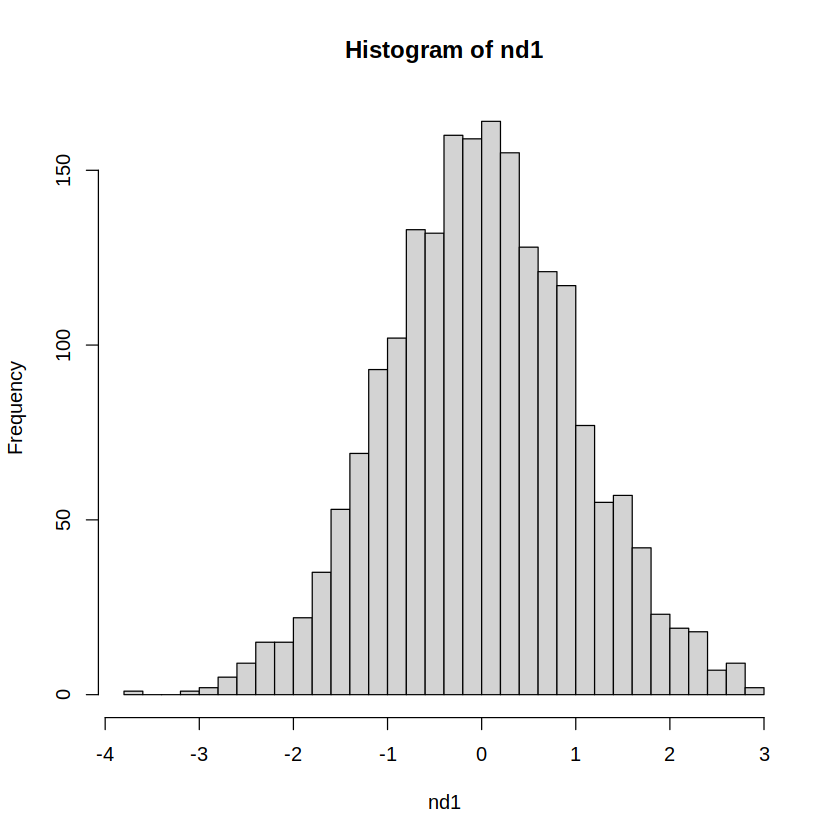
\includegraphics[width=0.7\textwidth]{4_attachments/figures/output23.png}
                        \caption{ Histogramme de la loi normale $\mathcal N(0,1)$ avec 20 classes}
                        \label{fig:fig3}
                    \end{figure}
                    
                \end{minipage}
              \end{table}

              La figure \ref{fig:fig1} représente un graphique obtenu à l'aide de la fonction \textbf{\textit{plot}}. 
              Ce graphique trace les valeurs de l'échantillon $nd1$ en fonction de leur indice. L'axe des abscisses ($x$) correspond aux indices des valeurs de l'échantillon, variant de $1$ à $n=2000$, tandis que l'axe des ordonnées ($y$) représente les valeurs de l'échantillon, lesquelles suivent une distribution normale.

              Ensuite, les graphiques des figures \ref{fig:fig2} et \ref{fig:fig3} sont tout deux obtenus à l'aide de la fonction \textbf{\textit{hist}}. Mais nous avons choisit manuellement le nombre de classes pour chaque histogramme pour la figure \ref{fig:fig3} grâce à la variable \textbf{\textit{breaks}}$=20$. Alors que pour le graphique de la figure \ref{fig:fig2}, nous avons laissé $R$ choisir automatiquement le nombre de classes.

        \subsubsection{Question 3 : Voir Code TP, section : Exercices sur la loi normale, Question 3 \cite{TP}}

            \begin{figure}[H]
                \centering
                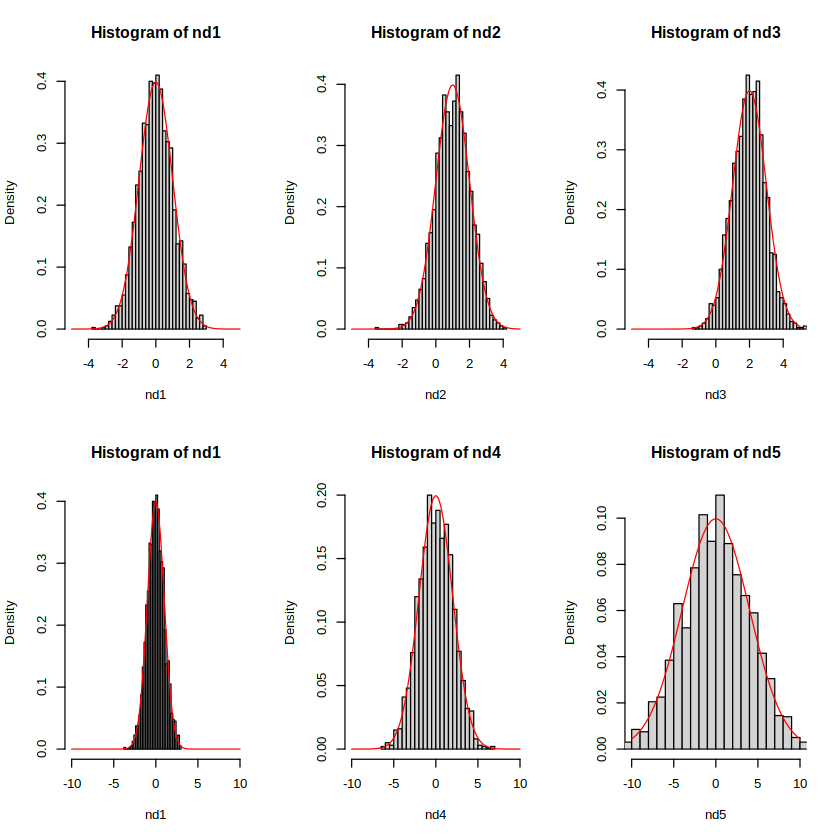
\includegraphics[width=0.38\textwidth]{4_attachments/figures/output24.png}
                \caption{Histogrammes des simulations avec leurs courbes de dentité théorique des échantillons: $\mathcal N(0,1)$, $\mathcal N(1,1)$ et $\mathcal N(2,1)$. Puis des échantillons $\mathcal N(0,1)$, $\mathcal N(0,2)$ et $\mathcal N(0,4)$}
                \label{fig:comparaison}
            \end{figure}

            \begin{center}
                \textit{Comparer les histogrammes des échantillons nd1, nd2 et nd3 : qu’est-ce qui change ?}
            \end{center}

            En examinant les trois premiers histogrammes de la figure \ref{fig:comparaison}, on constate qu'ils suivent une distribution normale avec des variances identiques mais des moyennes différentes. 
            Cela se traduit graphiquement par des courbes de densité centrées et symétriques autour de $x=0$ pour $\mathcal{N}(0,1)$, $x=1$ pour $\mathcal{N}(1,1)$, et $x=2$ pour $\mathcal{N}(2,1)$. 
            Les histogrammes de simulation se déplacent donc également vers la droite, en suivant la moyenne de chaque distribution.


            \begin{center}
                \textit{Comparer les histogrammes des échantillons nd1, nd4 et nd5 : qu’est-ce qui change ?}
            \end{center}
            On remarque cette fois-ci pour les 3 derniers histogrammes de la figure \ref{fig:comparaison} que les courbes de densité sont centrées autour de $x=0$ mais avec des variances différents.
            Graphiquement, cela se traduit par des courbes de densité plus ou moins étalées, plus ou moins aplaties, en fonction de l'variance de chaque distribution.
            Les histogrammes de simulation suivent donc la dispersion des valeurs autour de la moyenne. 


        \subsubsection{Question 4 : Voir Code TP, section : Exercices sur la loi normale, Question 4 \cite{TP}}
            \begin{figure}[H]
                \centering
                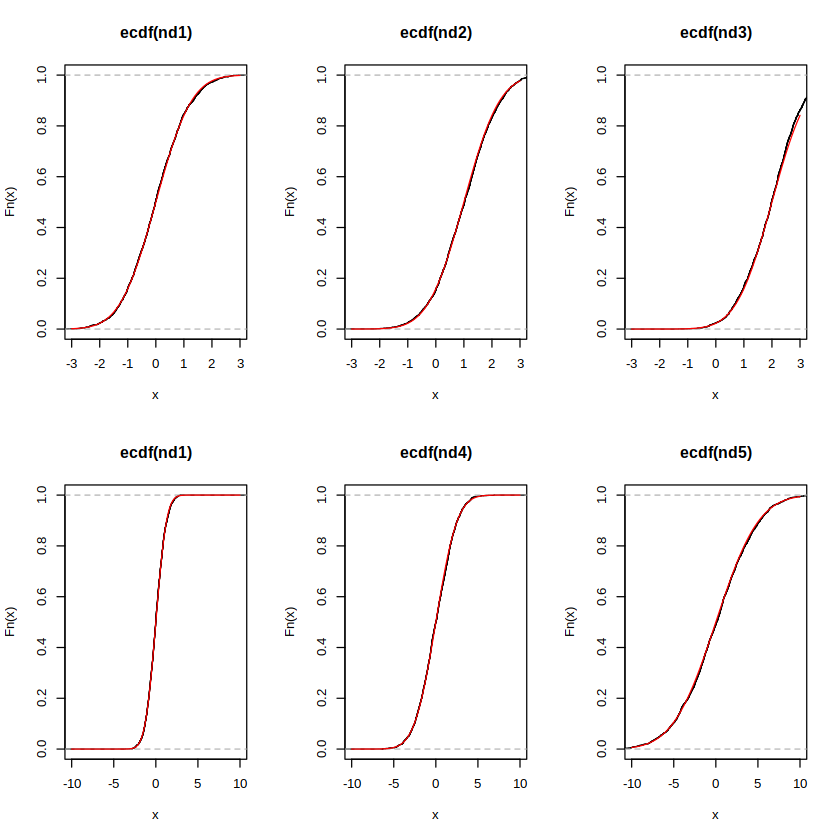
\includegraphics[width=0.35\textwidth]{4_attachments/figures/output25.png}
                \caption{Fonction de répartition simulées avec eur courbe théoriques des échantillons: $\mathcal N(0,1)$, $\mathcal N(1,1)$ et $\mathcal N(2,1)$. Puis des échantillons $\mathcal N(0,1)$, $\mathcal N(0,2)$ et $\mathcal N(0,4)$}
                \label{fig:comparaison}
            \end{figure}
            \begin{center}
                \textit{Comparer les fonctions de répartitions des échantillons nd1, nd2 et nd3 : qu’est-ce qui change ?}
            \end{center}
               En examinant les 3 premiers graphiques, nous observons que la forme de chaque courbe reste identique car l'variance est identique. 
               Mais leurs positions sur l'axe horizontal $x$ changent en fonction de la moyenne : plus la moyenne est élevée, plus la courbe est décalée vers la droite. 
               De plus, elles sont symétriques par rapport à l’axe des ordonnées de leur moyenne respective.
            \begin{center}
                \textit{Comparer les fonctions de répartitions des échantillons nd1, nd4 et nd5 : qu’est-ce qui change ?}
            \end{center}
            Pour des échantillons de même moyenne mais d'variances différents, les courbes sont toutes symétriques par rapport à l’axe des ordonnées de leur moyenne respective : $x=0$.
            Mais les courbes sont plus ou moins étalées, plus ou moins aplaties, en fonction de l'variance de chaque distribution.
        \subsubsection{Question 5 : Voir Code TP, section : Exercices sur la loi normale, Question 5 \cite{TP}}
            \begin{center}
                \textit{Donner ci-dessous la densité de la loi normale de moyenne 0 et de variance 1 :}
            \end{center}
            \[
                f(x) = \dfrac{1}{\sqrt{2\pi}}e^{-\frac{x^2}{2}}
            \]

            \begin{center}
                \textit{Quel est le lien entre la densité et la fonction de répartition ?}
            \end{center}

            La fonction de répartition $F(x)$ est la primitive de la densité $f(x)$, c'est-à-dire l'intégrale de $f(x)$ de $-\infty$ à $t$. 
            Elle permet de calculer la probabilité que la variable aléatoire $X \leq t$. (voir \cite{fct_repartition})
            \[
                F(t) = \int_{-\infty}^t f(x)\,dx
            \]
            \begin{table}[H]
                \centering
                \begin{minipage}{0.42\textwidth}
                    \begin{figure}[H]
                        \centering
                        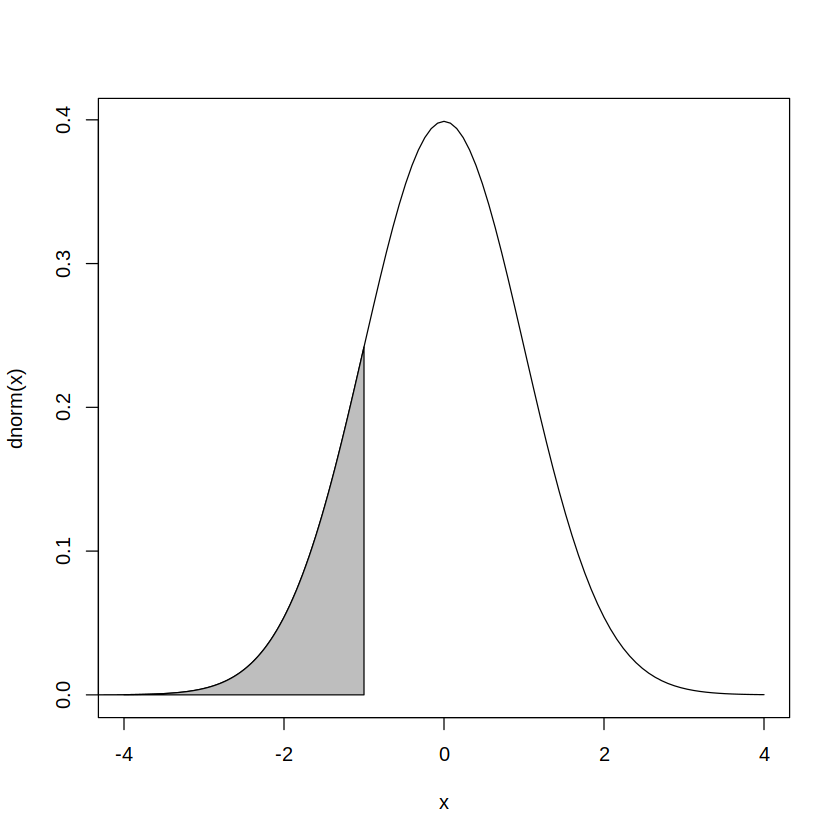
\includegraphics[width=0.45\textwidth]{4_attachments/figures/output26.png}
                        \caption{Courbe de densité de $\mathcal N(0,1)$ avec la zone de probabilité $P(X\leq -1)$}                
                        \label{fig:anal1}
                    \end{figure}
                \end{minipage}
                \hfill
                \begin{minipage}{0.42\textwidth}
                    \centering
                    \begin{figure}[H]
                        \centering
                        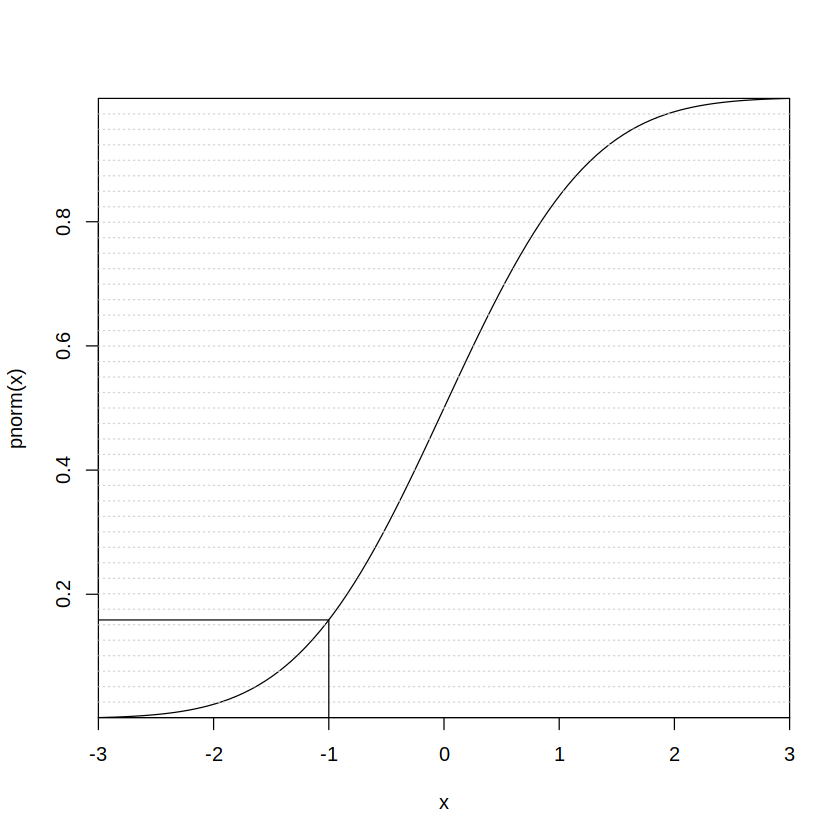
\includegraphics[width=0.45\textwidth]{4_attachments/figures/output27.png}
                        \caption{Fonction de répartition de la loi normale $\mathcal N(0,1)$ avec intersection en $x=-1$}              
                        \label{fig:anal2}
                    \end{figure}
                \end{minipage}
            \end{table}

            Les graphiques ci-dessus permettent de visualiser la probabilité $P(X\leq -1) = 0.1587$ pour la loi normale $\mathcal N(0,1)$.
            Dans le graphique de la figure \ref{fig:anal1}, la zone coloriée en gris représente l'aire sous la courbe de densité de la loi normale centrée réduite $\mathcal N(0,1)$ pour $x\leq -1$ qui est égal à $0.1587$.
            La figure \ref{fig:anal2} illustre la fonction de répartition de $\mathcal N(0,1)$, laquelle permet en lisant l'intersection de la courbe de répartition en $x=-1$ : $P(X\leq -1) = 0.1587$ 

        \subsubsection{Question 6}
            \begin{table}[H]
                \centering
                \begin{tabular}{|c|c|c|c|}
                    \hline
                    Aire de la figure & Pr représentée par l'aire & Ecriture avec F(t) & Valeur de pnorm \\
                    \hline
                    1 & $P(X\leq -1)$ & $F(-1)$ & 0.308 \\
                    2 & $P(X\leq 2)$ & $F(2)$ & 0.841 \\
                    3 & $P(X \geq 2)$ & $1-F(2)$ & 0.159 \\
                    4 & $P(-1 \leq X \leq 2)$ & $F(2)-F(-1)$ & 0.532 \\
                    \hline
                \end{tabular}
                \caption{Tableau de comparaison des valeurs de probabilités entre les fonctions de répartition et la fonction pnorm pour une loi normale $\mathcal N(0,4)$, \textbf{voir code annexe \ref{lst:q6}}}
                \label{tab:tab3}
            \end{table}

            \begin{center}
                \textit{Soit X une variable aléatoire gaussienne de moyenne 15 et de variance 9. Quelle est la  $Pr(X \leq 17)$ ?}
            \end{center}
            
            \noindent La fonction \textbf{\textit{pnorm(17,15,3)}} de paramètres $17$ ($x$), $15$ (moyenne) et $3$ (écart-type) permet de calculer la probabilité $Pr(X \leq 17)= 0.747$

            \begin{center}
                \textit{Quelle est $Pr(X>7)$ ?}
            \end{center}
            \noindent La fonction \textbf{\textit{1-pnorm(7,15,3)}} permet de calculer $Pr(X>7)= 0.996$

            \begin{center}
                \textit{Enfin quelle est la $Pr(7<X<15)$ ?}
            \end{center}
            \noindent La fonction \textbf{\textit{pnorm(15,15,3)-pnorm(7,15,3)}} permet de calculer $Pr(X>7)= 0.496$

    \subsection{Lien entre les lois normales}

    Soit $X$ une variable aléatoire distribuée suivant $\mathcal N(0,1)$.
    On souhaite montrer que les variables $X_1=X+1$, $X_2=X-1$, $X_3=2X$ et $X_4=X/2$ suivent aussi une loi normale. 
    Pour cela on simule un grand nombre de valeurs suivant la loi normale N(0,1) et l’on construit les nouvelles variables.

    \begin{figure}[H]
        \centering
        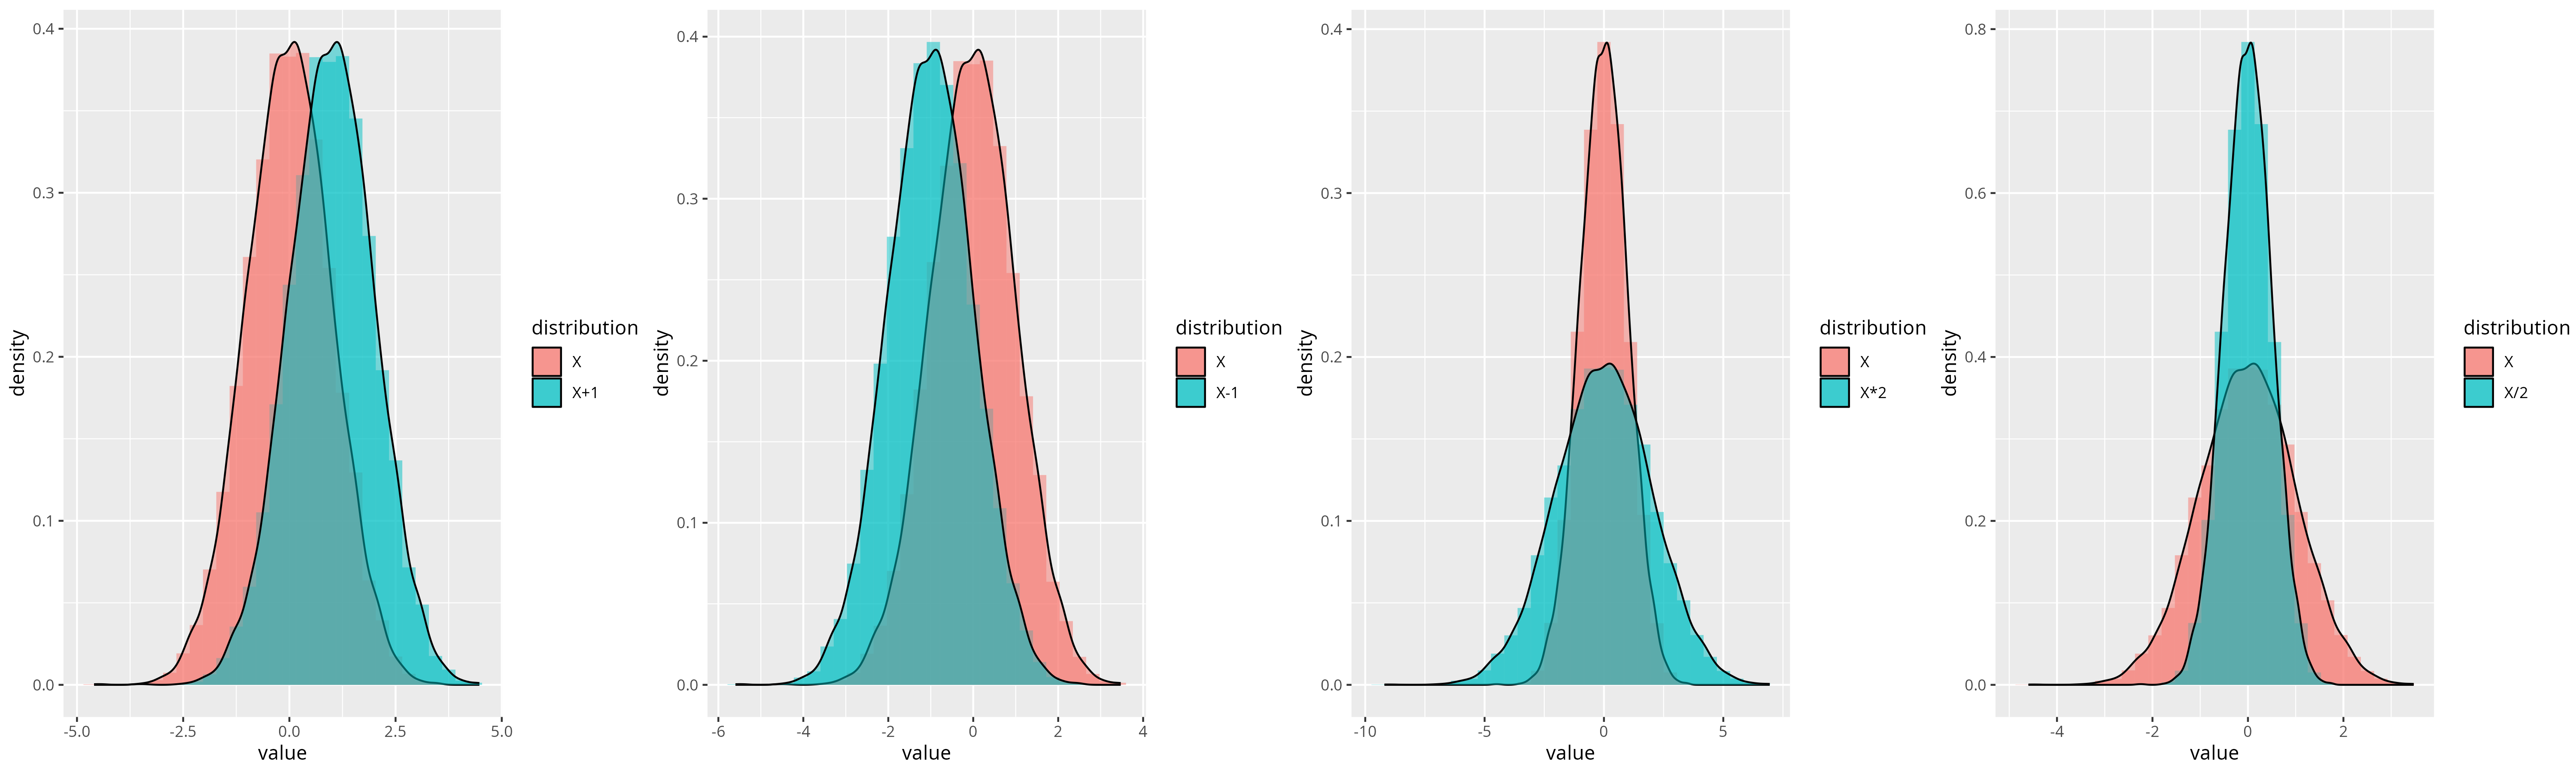
\includegraphics[width=1\textwidth]{4_attachments/figures/output28.png}
        \caption{Comparaison des lois normales $\mathcal N(0,1)$ avec les variables $X_1=X+1$, $X_2=X-1$, $X_3=2X$ et $X_4=X/2$ suivant une loi normale}                
        \label{fig:comparaison_loi_normales}
    \end{figure}

    Le graphique de la figure \ref{fig:comparaison_loi_normales} démontre que les variables $X_1=X+1$, $X_2=X-1$, $X_3=2X$ et $X_4=X/2$ suivent également une loi normale (\textbf{voir code annexe \ref{lst:lien_normales}}).

    \noindent Plus précisément, nous observons que $X_1$ suit la loi $\mathcal{N}(1,1)$, $X_2$ la loi $\mathcal{N}(-1,1)$, $X_3$ la loi $\mathcal{N}(0,2)$ et $X_4$ la loi $\mathcal{N}(0,0.5)$. 
    Ces résultats confirment ainsi que toute combinaison affine d'une variable normalement distribuée demeure normale, tout en modifiant la moyenne et la variance selon les opérations effectuées.

    \begin{center}
        \textit{Soit maintenant $Y$ une variable aléatoire de moyenne $4$ et de variance $3$, quelle est la distribution de la variable $Z=\frac{Y-2}{\sqrt{3}}$ ?}
    \end{center}

    \begin{figure}[H]
        \centering
        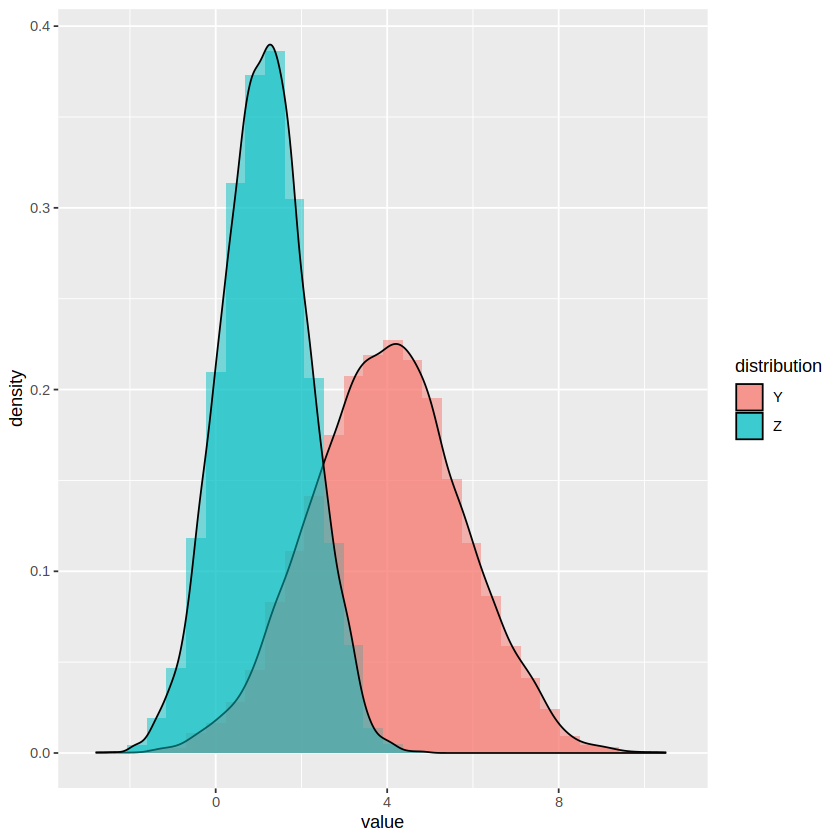
\includegraphics[width=0.32\textwidth]{4_attachments/figures/output29.png}
        \caption{Comparaison des lois normales $\mathcal N(4,3)$ avec la variable $Z=\frac{Y-2}{\sqrt{3}}$ suivant une loi normale}               
        \label{fig:comparaison_loi_normales}
    \end{figure}

    Nous remarquons que $Z$ suit une loi normale $\mathcal{N}(1,1)$. A noter que si $Z$ respectait le théorème de la loi centrée réduite $ Z^{*} = \dfrac{Y-\mu}{\sigma}= \dfrac{Y-4}{\sqrt{3}}$ alors $Z^{*}$ suivrait une loi normale $\mathcal{N}(0,1)$.
    \subsection{Sommes de variables aléatoires gaussiennes}

    \begin{center}
        \textit{Donner la loi de $X+Y$ et de $X-Y$ si $X\leadsto N(m_1,\sigma_1^2)$ et $Y\leadsto N(m_2,\sigma_2^2)$}
    \end{center}
    \begin{equation}
        X+Y\leadsto N(m_1+m_2,\sigma_1^2+\sigma_2^2) \quad \text{et} \quad X-Y\leadsto N(m_1-m_2,\sigma_1^2+\sigma_2^2)
        \label{eq:sommegaussiennes}
    \end{equation}

    \noindent \textbf{Voir code annexe \ref{lst:somme_gaussiennes} : Code : Sommes de variables aléatoires gaussiennes} et Code TP, section : Sommes de variables aléatoires gaussiennes \cite{TP}

      \begin{table}[H]
        \centering
        \begin{minipage}{0.28\textwidth}
            \centering
            \begin{figure}[H]
                \centering
                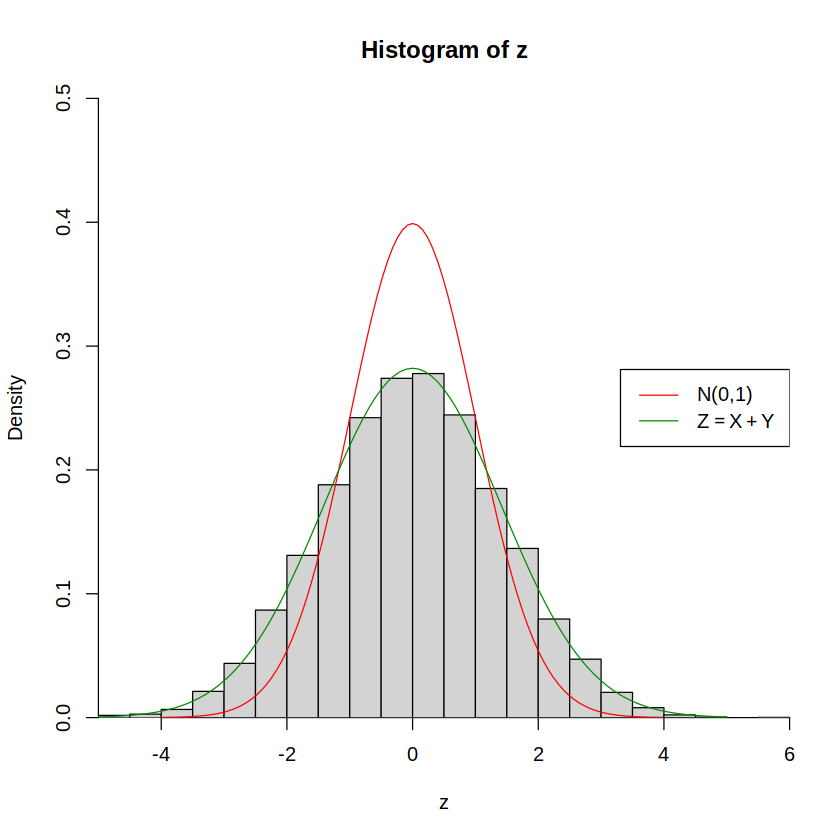
\includegraphics[width=0.80\textwidth]{4_attachments/figures/output31.png}
                \caption{Histogramme de la somme de 2 lois normales $\mathcal N(0,1)$}
                \label{fig:fig1}
            \end{figure}
         \end{minipage}
        \hfill
        \begin{minipage}{0.28\textwidth}
            \centering
            \begin{figure}[H]
                \centering
                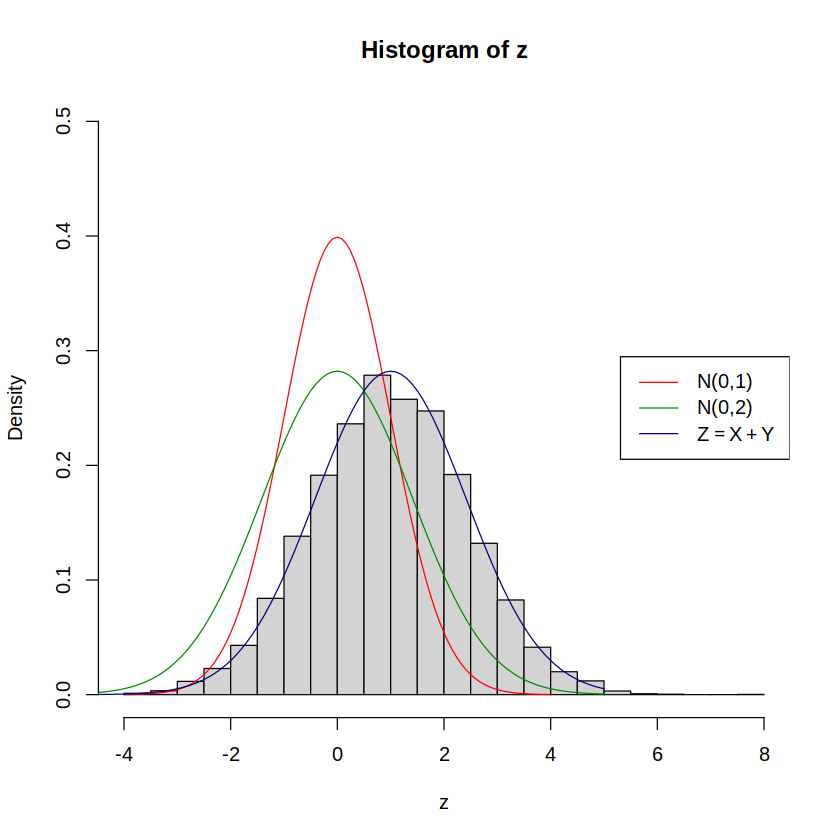
\includegraphics[width=0.80\textwidth]{4_attachments/figures/output32.png}
                \caption{Histogramme de la somme de 2 lois normales $\mathcal N(0,1)$ et $\mathcal N(1,1)$}
                \label{fig:fig2}
            \end{figure}
            
        \end{minipage}
        \hfill
        \begin{minipage}{0.28\textwidth}
            \centering
            \begin{figure}[H]
                \centering
                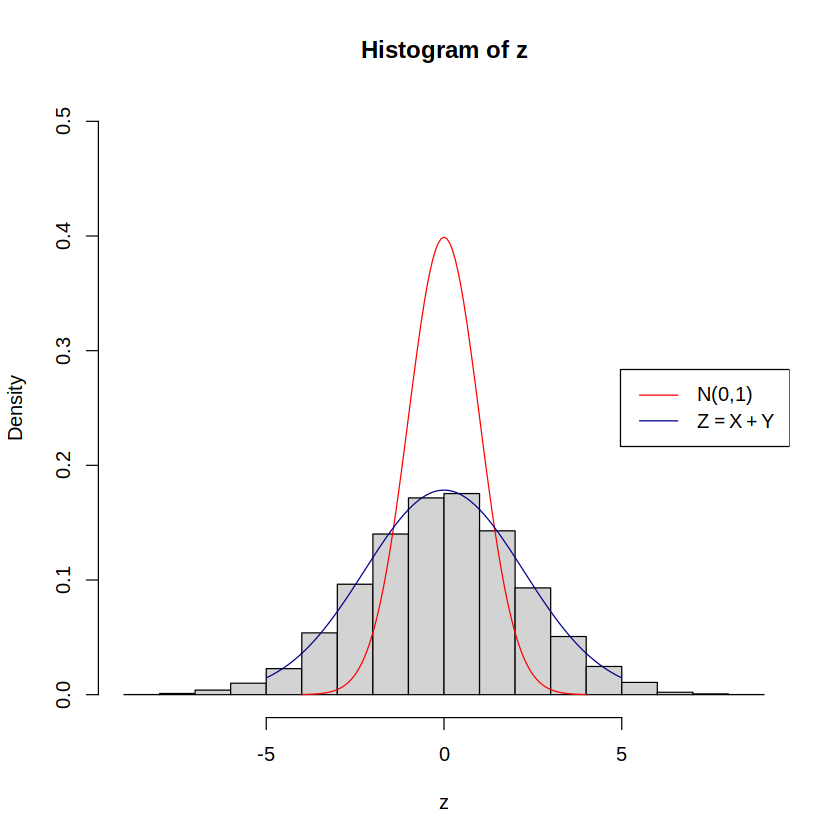
\includegraphics[width=0.80\textwidth]{4_attachments/figures/output33.png}
                \caption{Histogramme de la somme de 2 lois normales $\mathcal N(0,1)$ et $\mathcal N(0,2)$}
                \label{fig:fig3}
            \end{figure}
            
        \end{minipage}
      \end{table}
      \begin{center}
        \textit{Déduire de ce qui précède la loi de la variable $\bar{X}=\frac{1}{n}(X_1+X_2+X_3+...+X_n)$ où toutes les variables $X_i$ sont gaussiennes centrées réduites.}
        \end{center}
        \begin{equation}
            \bar{X} = \frac{1}{n}(X_1 + X_2 + \dots + X_n) \leadsto N\left( \frac{1}{n} \sum_{i=1}^{n} m_i, \frac{1}{n} \sum_{i=1}^{n} \sigma_i^2 \right)
            \label{eq:moyennegaussiennes}
        \end{equation}

    \noindent \textbf{Voir code annexe \ref{lst:mean_gaussiennes} : Code : Démonstration de la loi d'une moyenne de lois gaussienne $\bar{X}$}


    \subsection{Somme de carrés de variables gaussiennes centrées réduites}

    \begin{center}
        \textit{Trouver le nom de la nouvelle loi des carrés et comment on choisit ses paramètres?}
    \end{center}
    \begin{equation}
        X_1^2+X_2^2+X_3^2+...+X_n^2\leadsto \chi^2(n)
        \label{eq:eq_somme}
    \end{equation}

    Sur R, il faut utiliser la fonction \textbf{\textit{dchisq(n)}} pour avoir la distribution de la loi. Elle prend en paramètre $x$ la valeur à évaluer et $n$ le nombre de degrés de liberté (dans notre cas c'est l'index $n$ de l'équation \ref{eq:eq_somme}).

    \begin{table}[H]
        \centering
        \begin{minipage}{0.28\textwidth}
            \centering
            \begin{figure}[H]
                \centering
                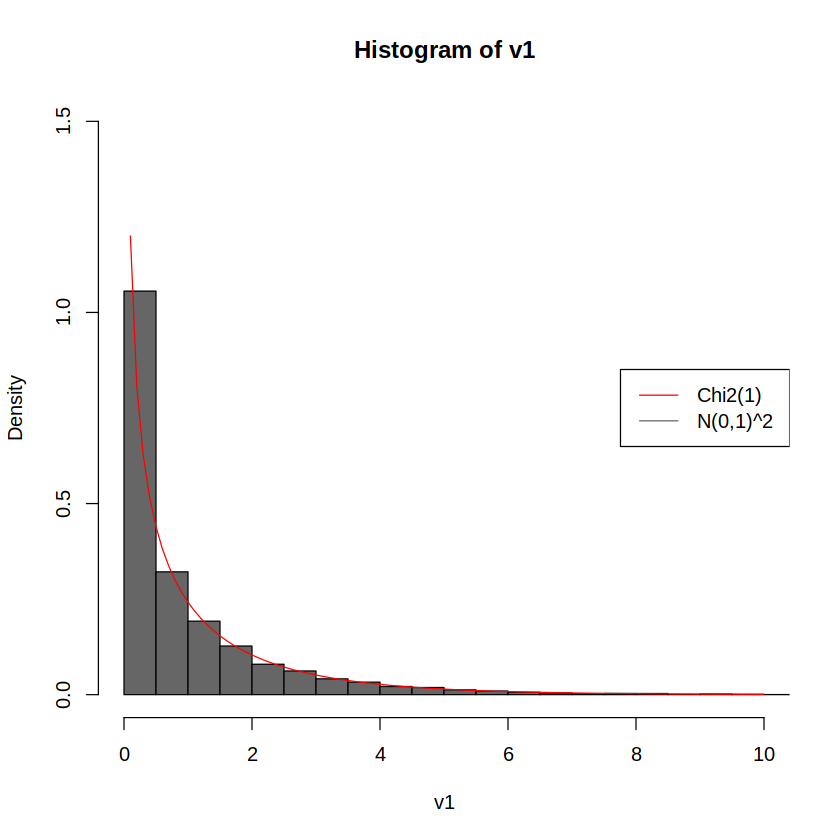
\includegraphics[width=0.80\textwidth]{4_attachments/figures/output41.png}
                \caption{Histogramme de la somme de carrés de 2 lois normales $\mathcal N(0,1)$}
                \label{fig:fig4}
            \end{figure}
         \end{minipage}
        \hfill
        \begin{minipage}{0.28\textwidth}
            \centering
            \begin{figure}[H]
                \centering
                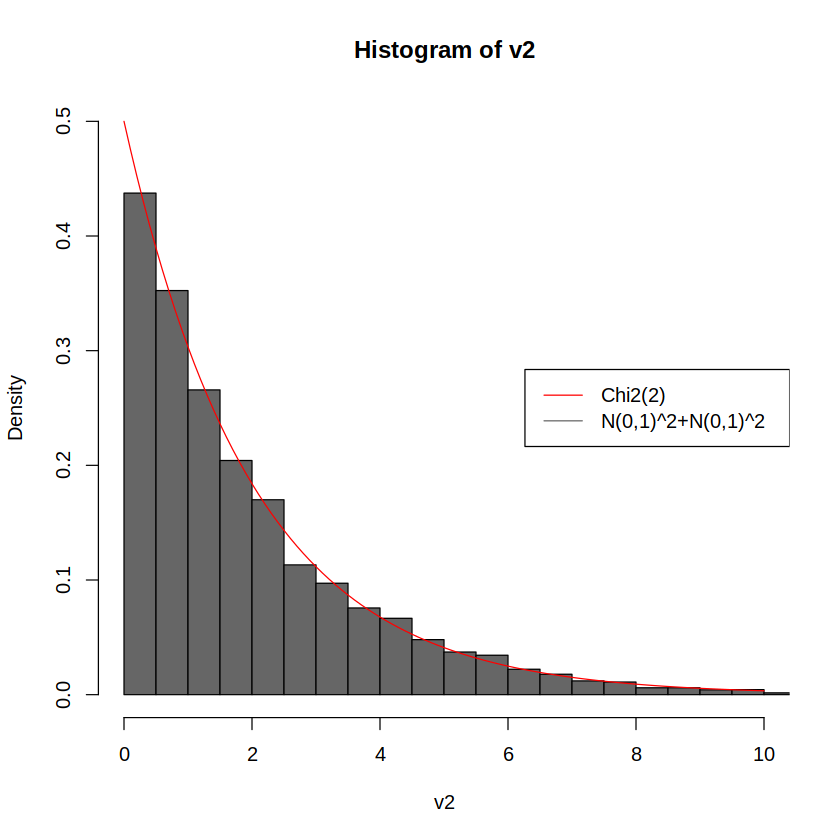
\includegraphics[width=0.80\textwidth]{4_attachments/figures/output42.png}
                \caption{Histogramme de la somme de carrés de 3 lois normales $\mathcal N(0,1)$}
                \label{fig:fig5}
            \end{figure}
            
        \end{minipage}
        \hfill
        \begin{minipage}{0.28\textwidth}
            \centering
            \begin{figure}[H]
                \centering
                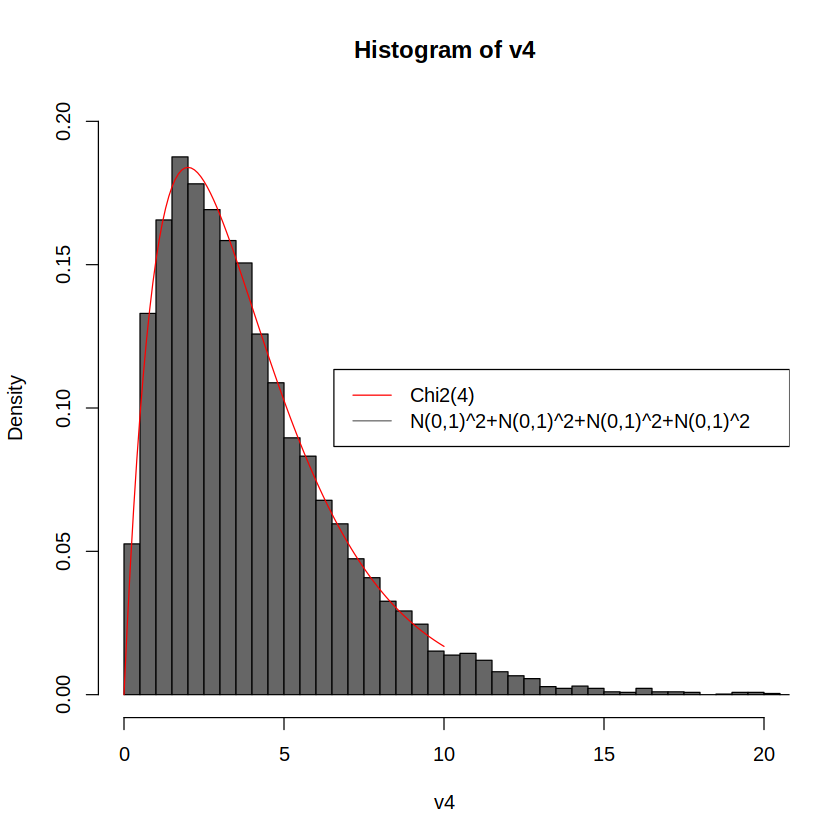
\includegraphics[width=0.80\textwidth]{4_attachments/figures/output43.png}
                \caption{Histogramme de la somme de carrés de 4 lois normales $\mathcal N(0,1)$}
                \label{fig:fig6}
            \end{figure}
            
        \end{minipage}
      \end{table}
    \subsection{Exercice}
        \noindent \textbf{Voir code annexe \ref{lst:exo} : Code : Exercice sur la loi normale}

        La taille $X$ d’un homme français tiré au sort dans la population est supposée suivre une loi normale de moyenne $172cm$ et de variance $196cm^2$.
        \begin{center}
            \textit{\textbf{Question 1} Quelle est la probabilité que $X$ soit inférieure à $160cm$ ?}
        \end{center}
        Pour calculer la probabilité que $X$ soit inférieure à 160 cm, nous devons calculer $P(X<160) = F(160)$ où $F$ est la fonction de répartition de la loi normale $\mathcal N(172,196)$.
        \[
            P(X<160) = F(160) = 0.196
        \]
        \begin{center}
            \textit{\textbf{Question 2} Quelle est la probabilité qu’un homme tiré au sort mesure plus de deux mètres ?}
        \end{center}
        Pour calculer la probabilité qu’un homme tiré au sort mesure plus de deux mètres, nous devons calculer $P(X>200) = 1-F(200)$ où $F$ est la fonction de répartition de la loi normale $\mathcal N(172,196)$.
        \[
            P(X>200) = 1-F(200) = 0.023
        \]
        \begin{center}
            \textit{\textbf{Question 3} Que vaut $P(165 < X < 185)$ ?}
        \end{center}
        Pour calculer la probabilité que $X$ soit comprise entre 165 et 185 cm, nous devons calculer $P(165<X<185) = F(185)-F(165)$ où $F$ est la fonction de répartition de la loi normale $\mathcal N(172,196)$.
        \[
            P(165<X<185) = F(185)-F(165) = 0.515
        \]

        \begin{center}
            \textit{\textbf{Question 4} La taille des femmes suit une loi gaussienne de moyenne $162cm$ et de variance $144cm^2$. Quelle est la probabilité qu’un homme tiré au sort soit plus grand qu’une femme choisie au hasard}
        \end{center}

        Pour calculer la probabilité qu’un homme tiré au sort soit plus grand qu’une femme choisie au hasard, nous devons calculer on défini $Z$ la variable aléatoire de la différence de taille entre un homme et une femme (voir équation de la somme des lois gaussiennes \ref{eq:sommegaussiennes}). 
        $X$ variable aléatoire de la taille d'un homme et $Y$ variable aléatoire de la taille d'une femme.
        \[
            Z = X - Y \leadsto \mathcal N(172-162,196+144) = \mathcal N(10,340)
        \]
        \[
            P(X>Y) = P(X-Y>0) = 1-F(0) = 0.706
        \]



    \subsection{Loi Exponentielle}
        On dit que X suit une loi exponentielle de paramètre $\lambda >0$, ce que l’on note $X\leadsto \mathcal E(\lambda)$ ssi sa fonction densité est : 
        \begin{equation}
            \forall x\in \mathbb R,\,f(x)=\left \lbrace 
            \begin{array}{cl}
                \lambda \exp(-\lambda x) & \text{si } x \geq 0 \\
                0 & \text {sinon}
                \end{array} \right.
            \label{eq:exp}
        \end{equation}

        \begin{center}
            \textit{Vérifier que la fonction $f$ est bien une densité de probabilité}
        \end{center}

        Pour vérifier que la fonction $f$ est bien une densité de probabilité, il faut vérifier que l'intégrale de $f$ sur $\mathbb R$ est égale à $1$.  La fonction $f$ doit également être positive sur $\mathbb R$ et continue.
        \[
            \int_{-\infty}^{+\infty} f(x)\,dx = \int_{0}^{+\infty} \lambda \exp(-\lambda x)\,dx = 1
        \]
        \textbf{Voir code annexe \ref{lst:exp} : Code : Vérification de la densité de probabilité de la loi exponentielle}

        Une simulation $S$ avec un échantillon $n=30$ et $\lambda = 0.001$ donnerait un histogramme avec une distribution exponentielle décroissante avec une espérance de $\mathbb{E}(S) \approx \frac{1}{0.001} \approx 1000$ et une variance de $\mathbb{V}(S) \approx \frac{1}{0.001^2} \approx 10^6$.
        Sa fonction de répartition est donnée par $F(x) = 1-\exp(-\lambda x)$ et sera quant à elle une fonction exponentielle croissante. (voir code TP, section : Loi Exponentielle \cite{TP})

\newpage